
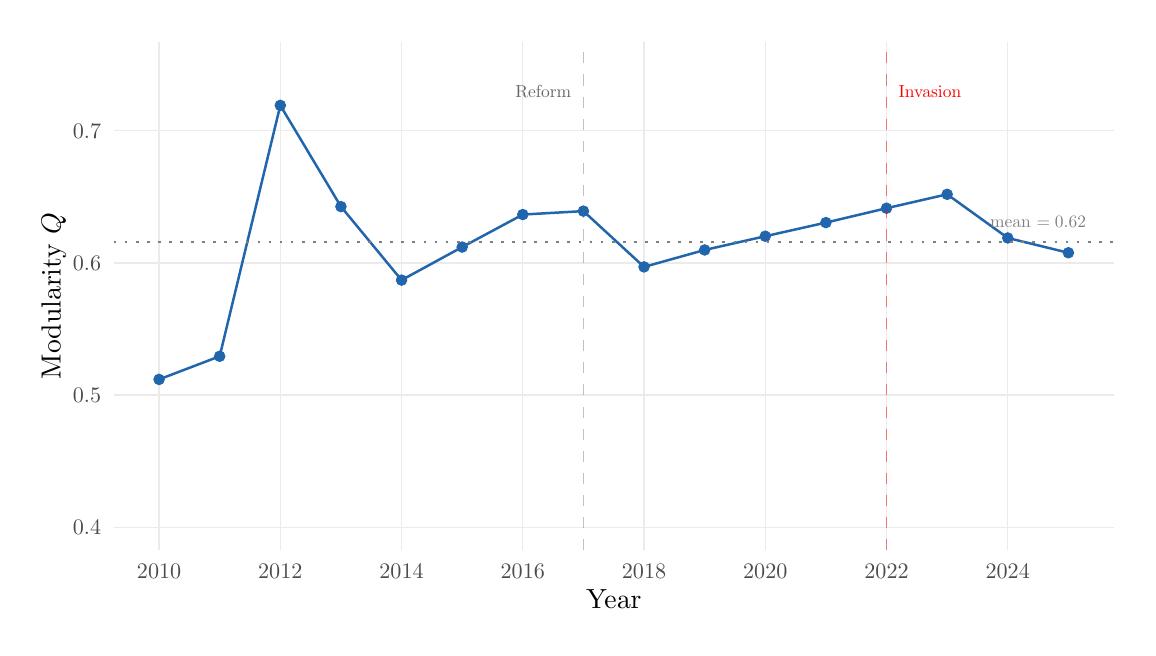
\begin{tikzpicture}[x=1pt,y=1pt]
\definecolor{fillColor}{RGB}{255,255,255}
\path[use as bounding box,fill=fillColor,fill opacity=0.00] (0,0) rectangle (397.48,216.81);
\begin{scope}
\path[clip] (  0.00,  0.00) rectangle (397.48,216.81);
\definecolor{fillColor}{RGB}{255,255,255}

\path[fill=fillColor] ( -0.00,  0.00) rectangle (397.48,216.81);
\end{scope}
\begin{scope}
\path[clip] ( 31.05, 27.90) rectangle (392.48,211.81);
\definecolor{drawColor}{gray}{0.92}

\path[draw=drawColor,line width= 0.5pt,line join=round] ( 31.05, 36.26) --
	(392.48, 36.26);

\path[draw=drawColor,line width= 0.5pt,line join=round] ( 31.05, 84.03) --
	(392.48, 84.03);

\path[draw=drawColor,line width= 0.5pt,line join=round] ( 31.05,131.80) --
	(392.48,131.80);

\path[draw=drawColor,line width= 0.5pt,line join=round] ( 31.05,179.57) --
	(392.48,179.57);

\path[draw=drawColor,line width= 0.5pt,line join=round] ( 47.48, 27.90) --
	( 47.48,211.81);

\path[draw=drawColor,line width= 0.5pt,line join=round] ( 91.29, 27.90) --
	( 91.29,211.81);

\path[draw=drawColor,line width= 0.5pt,line join=round] (135.10, 27.90) --
	(135.10,211.81);

\path[draw=drawColor,line width= 0.5pt,line join=round] (178.91, 27.90) --
	(178.91,211.81);

\path[draw=drawColor,line width= 0.5pt,line join=round] (222.72, 27.90) --
	(222.72,211.81);

\path[draw=drawColor,line width= 0.5pt,line join=round] (266.53, 27.90) --
	(266.53,211.81);

\path[draw=drawColor,line width= 0.5pt,line join=round] (310.34, 27.90) --
	(310.34,211.81);

\path[draw=drawColor,line width= 0.5pt,line join=round] (354.15, 27.90) --
	(354.15,211.81);
\definecolor{drawColor}{RGB}{33,102,172}

\path[draw=drawColor,line width= 0.9pt,line join=round] ( 47.48, 89.71) --
	( 69.38, 98.07) --
	( 91.29,188.74) --
	(113.20,152.15) --
	(135.10,125.59) --
	(157.01,137.53) --
	(178.91,149.28) --
	(200.82,150.52) --
	(222.72,130.36) --
	(244.63,136.48) --
	(266.53,141.45) --
	(288.44,146.37) --
	(310.34,151.57) --
	(332.25,156.59) --
	(354.15,140.82) --
	(376.06,135.47);
\definecolor{fillColor}{RGB}{33,102,172}

\path[draw=drawColor,line width= 0.3pt,line join=round,line cap=round,fill=fillColor] ( 47.48, 89.71) circle (  1.93);

\path[draw=drawColor,line width= 0.3pt,line join=round,line cap=round,fill=fillColor] ( 69.38, 98.07) circle (  1.93);

\path[draw=drawColor,line width= 0.3pt,line join=round,line cap=round,fill=fillColor] ( 91.29,188.74) circle (  1.93);

\path[draw=drawColor,line width= 0.3pt,line join=round,line cap=round,fill=fillColor] (113.20,152.15) circle (  1.93);

\path[draw=drawColor,line width= 0.3pt,line join=round,line cap=round,fill=fillColor] (135.10,125.59) circle (  1.93);

\path[draw=drawColor,line width= 0.3pt,line join=round,line cap=round,fill=fillColor] (157.01,137.53) circle (  1.93);

\path[draw=drawColor,line width= 0.3pt,line join=round,line cap=round,fill=fillColor] (178.91,149.28) circle (  1.93);

\path[draw=drawColor,line width= 0.3pt,line join=round,line cap=round,fill=fillColor] (200.82,150.52) circle (  1.93);

\path[draw=drawColor,line width= 0.3pt,line join=round,line cap=round,fill=fillColor] (222.72,130.36) circle (  1.93);

\path[draw=drawColor,line width= 0.3pt,line join=round,line cap=round,fill=fillColor] (244.63,136.48) circle (  1.93);

\path[draw=drawColor,line width= 0.3pt,line join=round,line cap=round,fill=fillColor] (266.53,141.45) circle (  1.93);

\path[draw=drawColor,line width= 0.3pt,line join=round,line cap=round,fill=fillColor] (288.44,146.37) circle (  1.93);

\path[draw=drawColor,line width= 0.3pt,line join=round,line cap=round,fill=fillColor] (310.34,151.57) circle (  1.93);

\path[draw=drawColor,line width= 0.3pt,line join=round,line cap=round,fill=fillColor] (332.25,156.59) circle (  1.93);

\path[draw=drawColor,line width= 0.3pt,line join=round,line cap=round,fill=fillColor] (354.15,140.82) circle (  1.93);

\path[draw=drawColor,line width= 0.3pt,line join=round,line cap=round,fill=fillColor] (376.06,135.47) circle (  1.93);
\definecolor{drawColor}{gray}{0.50}

\path[draw=drawColor,line width= 0.5pt,dash pattern=on 1pt off 3pt ,line join=round] ( 31.05,139.42) -- (392.48,139.42);
\definecolor{drawColor}{RGB}{102,102,102}

\path[draw=drawColor,draw opacity=0.40,line width= 0.5pt,dash pattern=on 4pt off 4pt ,line join=round] (200.82, 27.90) -- (200.82,211.81);
\definecolor{drawColor}{RGB}{255,0,0}

\path[draw=drawColor,draw opacity=0.50,line width= 0.5pt,dash pattern=on 4pt off 4pt ,line join=round] (310.34, 27.90) -- (310.34,211.81);
\definecolor{drawColor}{gray}{0.40}

\node[text=drawColor,anchor=base east,inner sep=0pt, outer sep=0pt, scale=  0.63] at (196.43,191.74) {Reform};
\definecolor{drawColor}{RGB}{255,0,0}

\node[text=drawColor,anchor=base west,inner sep=0pt, outer sep=0pt, scale=  0.63] at (314.72,191.74) {Invasion};
\definecolor{drawColor}{gray}{0.50}

\node[text=drawColor,anchor=base,inner sep=0pt, outer sep=0pt, scale=  0.63] at (365.10,144.43) {mean $= 0.62$};
\end{scope}
\begin{scope}
\path[clip] (  0.00,  0.00) rectangle (397.48,216.81);
\definecolor{drawColor}{gray}{0.30}

\node[text=drawColor,anchor=base east,inner sep=0pt, outer sep=0pt, scale=  0.80] at ( 26.55, 33.50) {0.4};

\node[text=drawColor,anchor=base east,inner sep=0pt, outer sep=0pt, scale=  0.80] at ( 26.55, 81.27) {0.5};

\node[text=drawColor,anchor=base east,inner sep=0pt, outer sep=0pt, scale=  0.80] at ( 26.55,129.04) {0.6};

\node[text=drawColor,anchor=base east,inner sep=0pt, outer sep=0pt, scale=  0.80] at ( 26.55,176.81) {0.7};
\end{scope}
\begin{scope}
\path[clip] (  0.00,  0.00) rectangle (397.48,216.81);
\definecolor{drawColor}{gray}{0.30}

\node[text=drawColor,anchor=base,inner sep=0pt, outer sep=0pt, scale=  0.80] at ( 47.48, 17.89) {2010};

\node[text=drawColor,anchor=base,inner sep=0pt, outer sep=0pt, scale=  0.80] at ( 91.29, 17.89) {2012};

\node[text=drawColor,anchor=base,inner sep=0pt, outer sep=0pt, scale=  0.80] at (135.10, 17.89) {2014};

\node[text=drawColor,anchor=base,inner sep=0pt, outer sep=0pt, scale=  0.80] at (178.91, 17.89) {2016};

\node[text=drawColor,anchor=base,inner sep=0pt, outer sep=0pt, scale=  0.80] at (222.72, 17.89) {2018};

\node[text=drawColor,anchor=base,inner sep=0pt, outer sep=0pt, scale=  0.80] at (266.53, 17.89) {2020};

\node[text=drawColor,anchor=base,inner sep=0pt, outer sep=0pt, scale=  0.80] at (310.34, 17.89) {2022};

\node[text=drawColor,anchor=base,inner sep=0pt, outer sep=0pt, scale=  0.80] at (354.15, 17.89) {2024};
\end{scope}
\begin{scope}
\path[clip] (  0.00,  0.00) rectangle (397.48,216.81);
\definecolor{drawColor}{RGB}{0,0,0}

\node[text=drawColor,anchor=base,inner sep=0pt, outer sep=0pt, scale=  1.00] at (211.77,  6.94) {Year};
\end{scope}
\begin{scope}
\path[clip] (  0.00,  0.00) rectangle (397.48,216.81);
\definecolor{drawColor}{RGB}{0,0,0}

\node[text=drawColor,rotate= 90.00,anchor=base,inner sep=0pt, outer sep=0pt, scale=  1.00] at ( 11.89,119.85) {Modularity $Q$};
\end{scope}
\end{tikzpicture}

